\section{Einleitung}

Es gibt eine breite Auswahl verschiedener elektrischer Motortypen für die verschiedensten Anwendungsbereiche. Von der Zeitanzeige am Handgelenk über den Antrieb eines Bohrers bis hin zur Bewegung von schwersten Lasten in der Industrie gibt es für viele Applikationen den richtigen Motortyp mit den entsprechenden Eigenschaften.

Ein besonders vielfältiger Motorentyp ist der bürstenlose Gleichstrommotor oder kurz BLDC-Motor (aus dem englischen: \glqq{}Brushless direct current\grqq{}-Motor). Dieser Motorentyp erfreut sich seit seiner Erfindung einer wachsenden Beliebtheit (siehe Abbildung~\ref{fig:Statistik}).

\begin{figure}[h]
  \centering
  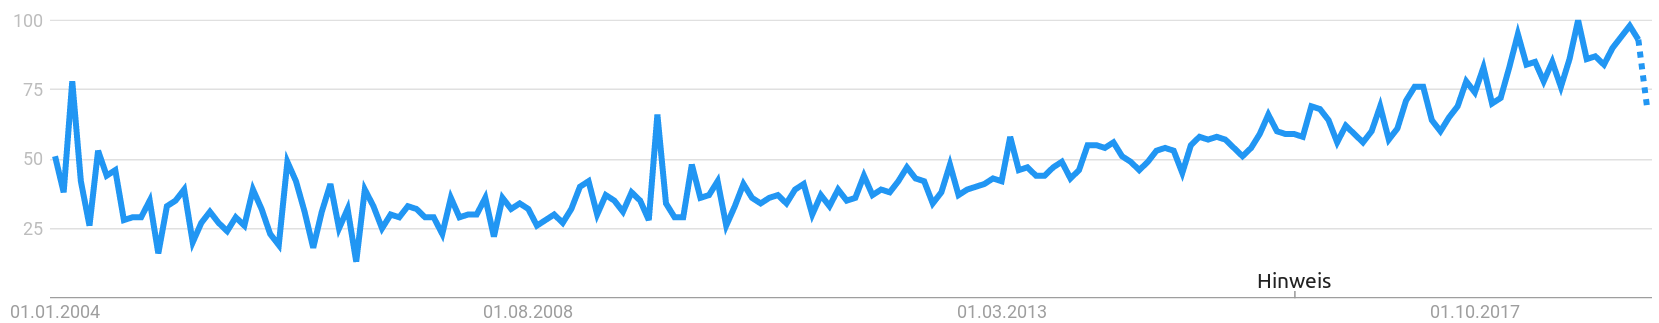
\includegraphics[width=\textwidth]{GoogleTrends_Statistik}
  \caption[Anzahl Google-Suchanfragen]{Anzahl der Google-Suchanfragen seit 2004. Wert von 100 entspricht der höchsten Beliebtheit innerhalb des angefragten Zeitraums (Quelle: Google Trends, Suchbegriff: \glqq{}bldc motor\grqq{})}
  \label{fig:Statistik}
\end{figure}

Der bürstenlose Gleichstrommotor soll in dieser Arbeit zunächst vom bürstenbehafteten Gleichstrommotor abgegrenzt und einige seiner charakteristischen Eigenschaften und Vorteile genannt werden. Es folgt eine Ausdifferenzierung verschiedener Ausführungen, gefolgt von den typischen Anwendungsfeldern dieses Motorentyps, sowie eines ausführlichen Anwendungsbeispiels.

Ziel dieser Arbeit ist es somit, den bürstenlosen Gleichstrommotor in das weite Feld der Aktorikapplikationen einzuordnen und seine Vorteile und Stärken hervorzuheben. Zudem kann die genaue Abgrenzung der verschiedenen Bauformen eine Hilfestellung in der Auswahl eines BLDC-Motoren bieten. Die Arbeit schließt mit einem Fazit.

%%% Local Variables:
%%% mode: latex
%%% TeX-master: "BLDC"
%%% End:
